\documentclass{ximera}

%% You can put user macros here
%% However, you cannot make new environments

\listfiles

\graphicspath{{./}{firstExample/}{secondExample/}}

\usepackage{tikz}
\usepackage{tkz-euclide}
\usepackage{tikz-3dplot}
\usepackage{tikz-cd}
\usetikzlibrary{shapes.geometric}
\usetikzlibrary{arrows}
\usetikzlibrary{decorations.pathmorphing,patterns}
\usetkzobj{all}
\pgfplotsset{compat=1.13} % prevents compile error.

\renewcommand{\vec}[1]{\mathbf{#1}}
\newcommand{\RR}{\mathbb{R}}
\newcommand{\dfn}{\textit}
\newcommand{\dotp}{\cdot}
\newcommand{\id}{\text{id}}
\newcommand\norm[1]{\left\lVert#1\right\rVert}
 
\newtheorem{general}{Generalization}
\newtheorem{initprob}{Exploration Problem}

\tikzstyle geometryDiagrams=[ultra thick,color=blue!50!black]

\usepackage{mathtools}

\title{Constant Coefficient Homogeneous Equations}


\begin{document}

\begin{abstract}
We examine the various possibilities for types of solutions when solving constant coefficient homogeneous equations.
\end{abstract}

\maketitle

\section*{Constant Coefficient Homogeneous Equations}

If $a,b$, and $c$ are real constants and $a\neq 0$, then
$$
ay''+by'+cy=F(x)
$$
 is said to be a \textit{constant coefficient
 equation}.
In this section we  consider the homogeneous constant
coefficient equation
\begin{equation} \label{eq:5.2.1}
ay''+by'+cy=0.
\end{equation}
As we'll see, all solutions of \eqref{eq:5.2.1} are defined on
$(-\infty,\infty)$.  This being the case, we'll omit references to the
interval on which solutions are defined, or on which a given set of
solutions is a fundamental set, etc., since the interval will always
be $(-\infty,\infty)$.

The key to solving \eqref{eq:5.2.1} is  that if
 $y=e^{rx}$ where $r$ is a constant  then the left side of
\eqref{eq:5.2.1} is a  multiple of $e^{rx}$;   thus, if $y=e^{rx}$
 then $y'=re^{rx}$ and $y''=r^2e^{rx}$, so
\begin{equation} \label{eq:5.2.2}
ay''+by'+cy=ar^2e^{rx}+bre^{rx}+ce^{rx}=(ar^2+br+c)e^{rx}.
\end{equation}
The quadratic polynomial
$$
p(r)=ar^2+br+c
$$
is  the \textit{characteristic polynomial} of \eqref{eq:5.2.1}, and
$p(r)=0$
is the \textit{characteristic equation}.
From \eqref{eq:5.2.2} we can see that $y=e^{rx}$ is a solution of
\eqref{eq:5.2.1}  if and only if $p(r)=0$.

The roots of the characteristic equation are given by the quadratic
formula
\begin{equation} \label{eq:5.2.3}
r=\frac{-b\pm\sqrt{b^2-4ac}}{2a}.
\end{equation}
We consider three cases:\\
Case 1. $b^2-4ac>0$, so the characteristic equation has two
distinct real roots.\\
Case 2. $b^2-4ac=0$, so the characteristic equation has a
repeated real root.\\
Case 3. $b^2-4ac<0$, so the characteristic equation has
complex roots.

In each case we'll start with an example.

\subsection*{Case 1: Distinct Real Roots}

\begin{example}\label{example:5.2.1}
\begin{enumerate}
    \item \label{item:5.2.1a}%(a)
Find the general solution of
\begin{equation} \label{eq:5.2.4}
y''+6y'+5y=0.
\end{equation}

\item \label{item:5.2.1b}%(b)
Solve the initial value problem
\begin{equation} \label{eq:5.2.5}
y''+6y'+5y=0, \quad   y(0)=3,\;  y'(0)=-1.
\end{equation}
\end{enumerate}

\begin{explanation}
\ref{item:5.2.1a}   The characteristic
polynomial of
 \eqref{eq:5.2.4} is
$$
p(r)=r^2+6r+5=(r+1)(r+5).
$$
Since $p(-1)=p(-5)=0$,  $y_1=e^{-x}$ and $y_2=e^{-5x}$
are solutions of \eqref{eq:5.2.4}. Since $y_2/y_1=e^{-4x}$  is
nonconstant, \ref{thmtype:5.1.6} implies that the general solution
of \eqref{eq:5.2.4} is
\begin{equation} \label{eq:5.2.6}
y=c_1e^{-x}+c_2e^{-5x}.
\end{equation}

\ref{item:5.2.1b} We  must determine $c_1$ and $c_2$
in  \eqref{eq:5.2.6} so that $y$ satisfies the initial conditions in
 \eqref{eq:5.2.5}. Differentiating  \eqref{eq:5.2.6} yields
\begin{equation} \label{eq:5.2.7}
y'=-c_1e^{-x}-5c_2e^{-5x}.
\end{equation}
Imposing the initial conditions $y(0)=3,\, y'(0)=-1$ in \eqref{eq:5.2.6}
and \eqref{eq:5.2.7} yields
$$\begin{array}{rcr}
c_1+c_2 & = & 3\\
-c_1-5c_2 & = & -1.
\end{array}$$
 The solution of this system is $c_1=7/2,c_2=-1/2$.  Therefore
the solution of  \eqref{eq:5.2.5} is
$$
y=\frac{7}{2}e^{-x}-\frac{1}{2}e^{-5x}.
$$
 the figure below is a graph
of this solution.

\begin{image}
 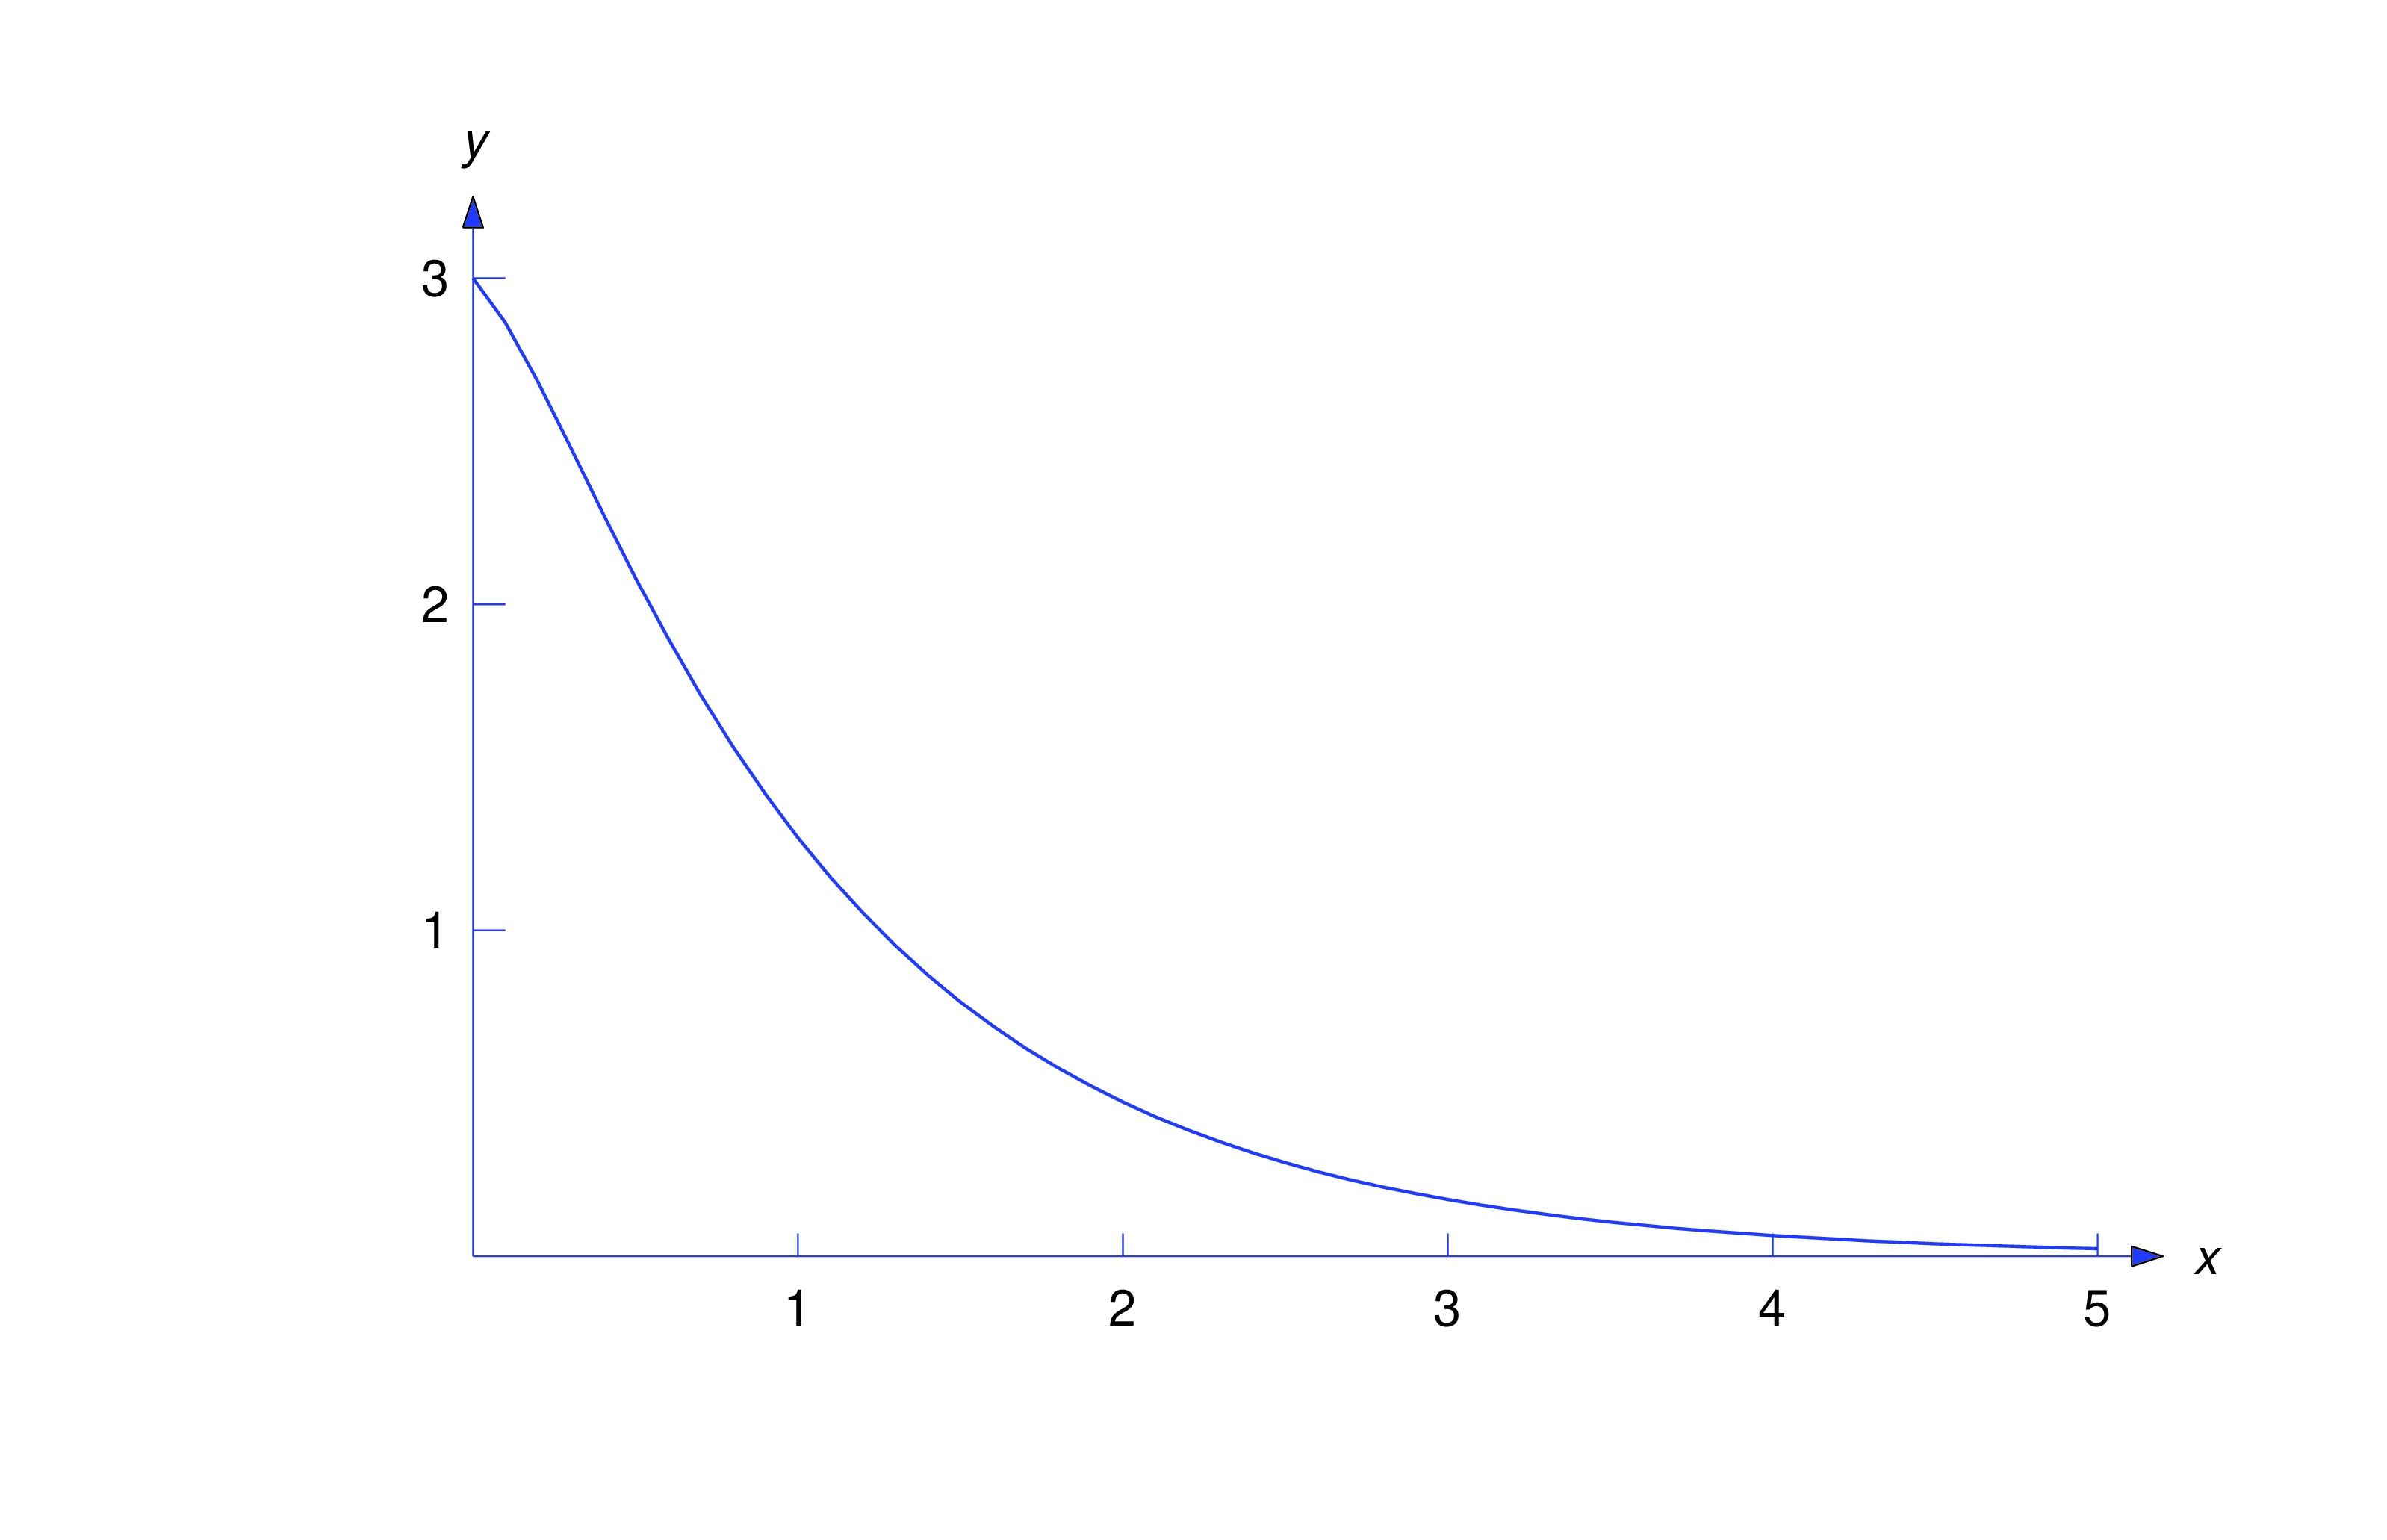
\includegraphics[height=1.5in]{fig050201.jpg}
\end{image}

\end{explanation}
\end{example}

% \begin{figure}[tbp]
%   \centering
%   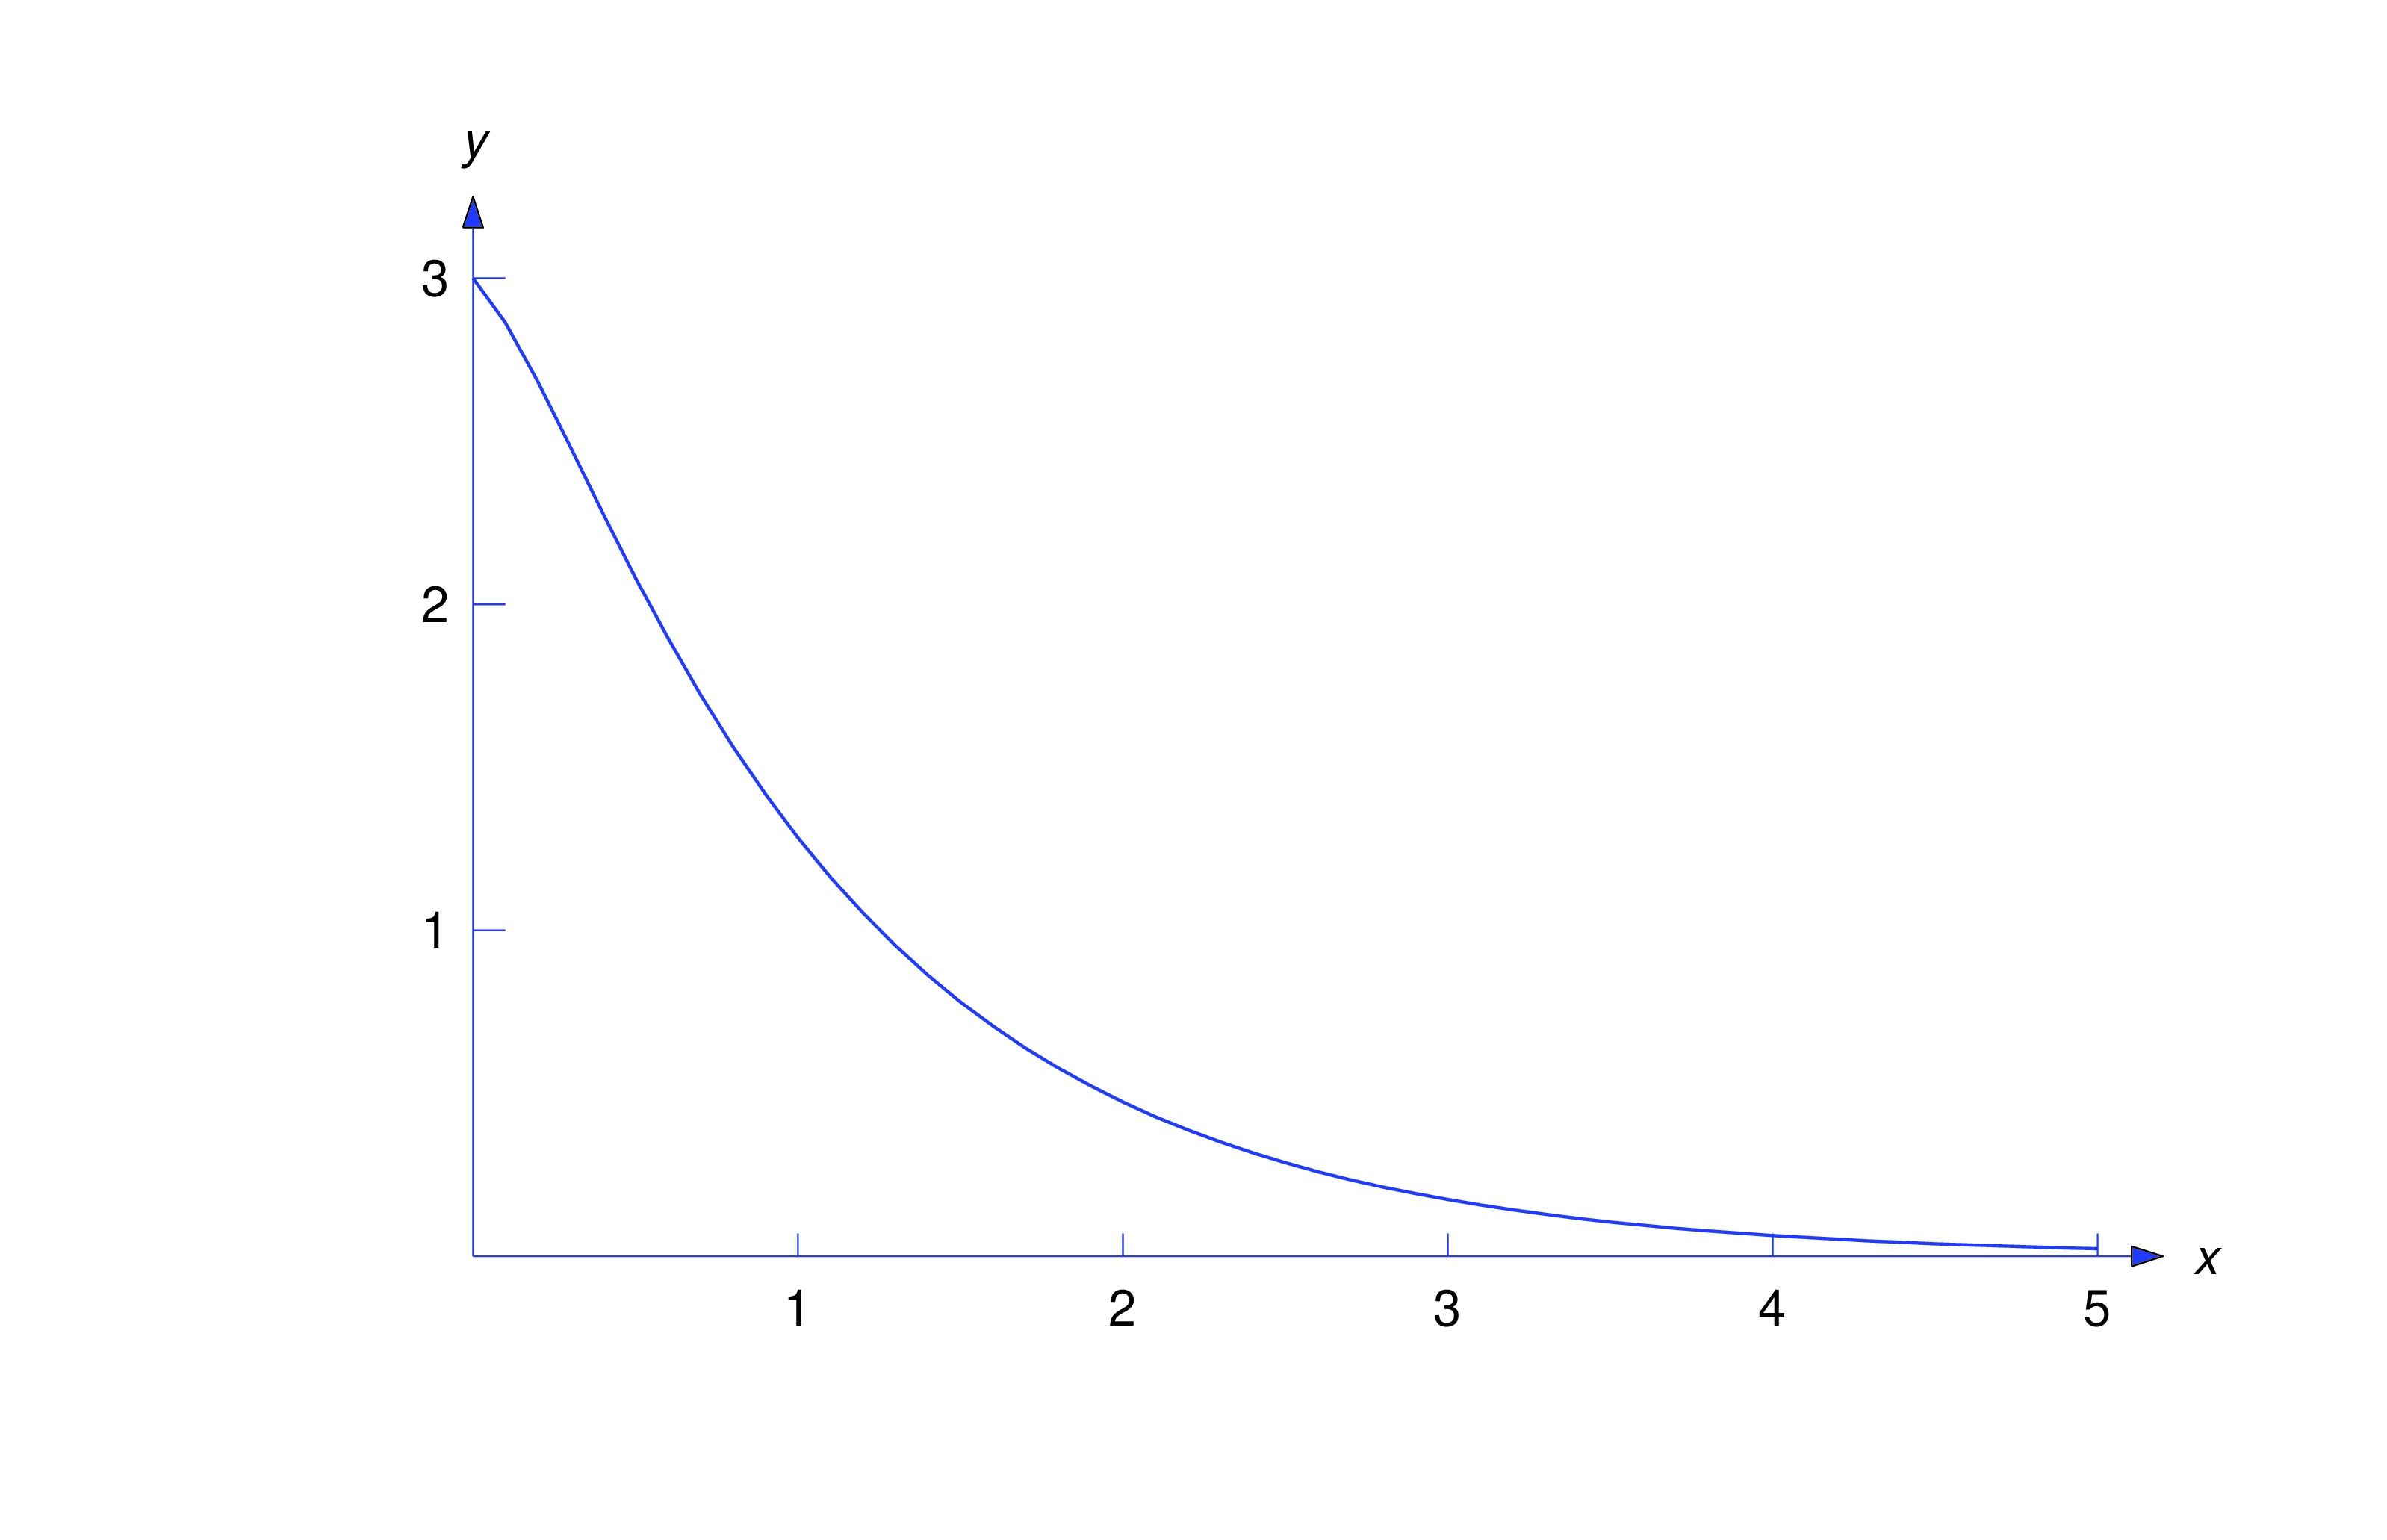
\includegraphics[bb=-78 148 689 643,width=5.67in,height=3.66in,keepaspectratio]{fig050201}
% \color{blue}
%   \caption{$y=\dst{{7\over2}e^{-x}-{1\over2}e^{-5x}}$ }
%   \label{figure:5.2.1}
% \end{figure}

If the characteristic equation has arbitrary distinct real roots
$r_1$ and $r_2$, then
$y_1=e^{r_1x}$ and $y_2=e^{r_2x}$  are  solutions of $ay''+by'+cy=0$.
Since $y_2/y_1=e^{(r_2-r_1)x}$ is nonconstant, Theorem~\ref{thmtype:5.1.6}
 implies that  $\{y_1,y_2\}$ is a fundamental
set of solutions of $ay''+by'+cy=0$.

\subsection*{Case 2: A Repeated Real Root}

\begin{example}\label{example:5.2.2}
\begin{enumerate}
\item\label{item:5.2.2a}%(a)
Find the general solution of
\begin{equation} \label{eq:5.2.8}
y''+6y'+9y=0.
\end{equation}

\item\label{item:5.2.2b}%(b)
Solve the initial value problem
\begin{equation} \label{eq:5.2.9}
y''+6y'+9y=0, \quad   y(0)=3,  y'(0)=-1.
\end{equation}
\end{enumerate}

\begin{explanation}
\ref{item:5.2.2a}  The characteristic polynomial of
 \eqref{eq:5.2.8} is
$$
p(r)=r^2+6r+9=(r+3)^2,
$$
so the characteristic equation has the repeated real root $r_1=-3$.
Therefore $y_1=e^{-3x}$ is a solution of \eqref{eq:5.2.8}. Since the
characteristic equation has no other roots, \eqref{eq:5.2.8}
has no other  solutions of the form $e^{rx}$.
 We  look for  solutions of the form
$y=uy_1=ue^{-3x}$,
where $u$ is a function that we'll now
determine.
% (This should remind you of the method of variation of parameters
% used in Module \ref{Module }%Section~2.1
% to solve the nonhomogeneous
% equation $y'+p(x)y=f(x)$, given a solution $y_1$ of the complementary
% equation $y'+p(x)y=0$.  It's also a special case of a method called
% \textit{reduction of order} that we'll study in Module \ref{Module 6}.%Section~5.6.
% For other ways to obtain a second solution of \eqref{eq:5.2.8} that's
% not a multiple of $e^{-3x}$, see
% Exercises~5.1.~\hspace*{-3pt}\ref{exer:5.1.9},
% 5.1.~\hspace*{-3pt}\ref{exer:5.1.12}, and \ref{exer:5.2.33}.

If $y=ue^{-3x}$, then
$$
y'=u'e^{-3x}-3ue^{-3x}\quad\mbox{and}\quad
y''=u''e^{-3x}-6u'e^{-3x}+9ue^{-3x},
$$
so
\begin{eqnarray*}
y''+6y'+9y&=&e^{-3x}\left[(u''-6u'+9u)+6(u'-3u)+9u\right]\\
&=&e^{-3x}\left[u''-(6-6)u'+(9-18+9)u\right]=u''e^{-3x}.
\end{eqnarray*}
Therefore $y=ue^{-3x}$ is a solution of \eqref{eq:5.2.8} if and only if
$u''=0$, which is equivalent to $u=c_1+c_2x$, where $c_1$ and $c_2$
are constants. Therefore any function of the form
\begin{equation} \label{eq:5.2.10}
y=e^{-3x}(c_1+c_2x)
\end{equation}
is  a solution of \eqref{eq:5.2.8}.
Letting $c_1=1$ and $c_2=0$  yields the solution
 $y_1=e^{-3x}$ that we already knew. Letting $c_1=0$ and $c_2=1$
yields the second solution $y_2=xe^{-3x}$. Since
$y_2/y_1=x$
is nonconstant, \ref{thmtype:5.1.6} implies that   $\{y_1,y_2\}$ is
fundamental set of solutions of \eqref{eq:5.2.8}, and \eqref{eq:5.2.10}
is the general solution.

\ref{item:5.2.2b}  Differentiating   \eqref{eq:5.2.10} yields
\begin{equation} \label{eq:5.2.11}
y'=-3e^{-3x}(c_1+c_2x)+c_2e^{-3x}.
\end{equation}
Imposing the initial conditions $y(0)=3,\, y'(0)=-1$ in \eqref{eq:5.2.10}
and \eqref{eq:5.2.11} yields $c_1=3$ and $-3c_1+c_2=-1$, so
$c_2=8$. Therefore the solution of \eqref{eq:5.2.9} is
$$
y=e^{-3x}(3+8x).
$$
The figure below is a graph of this solution.

\begin{image}
 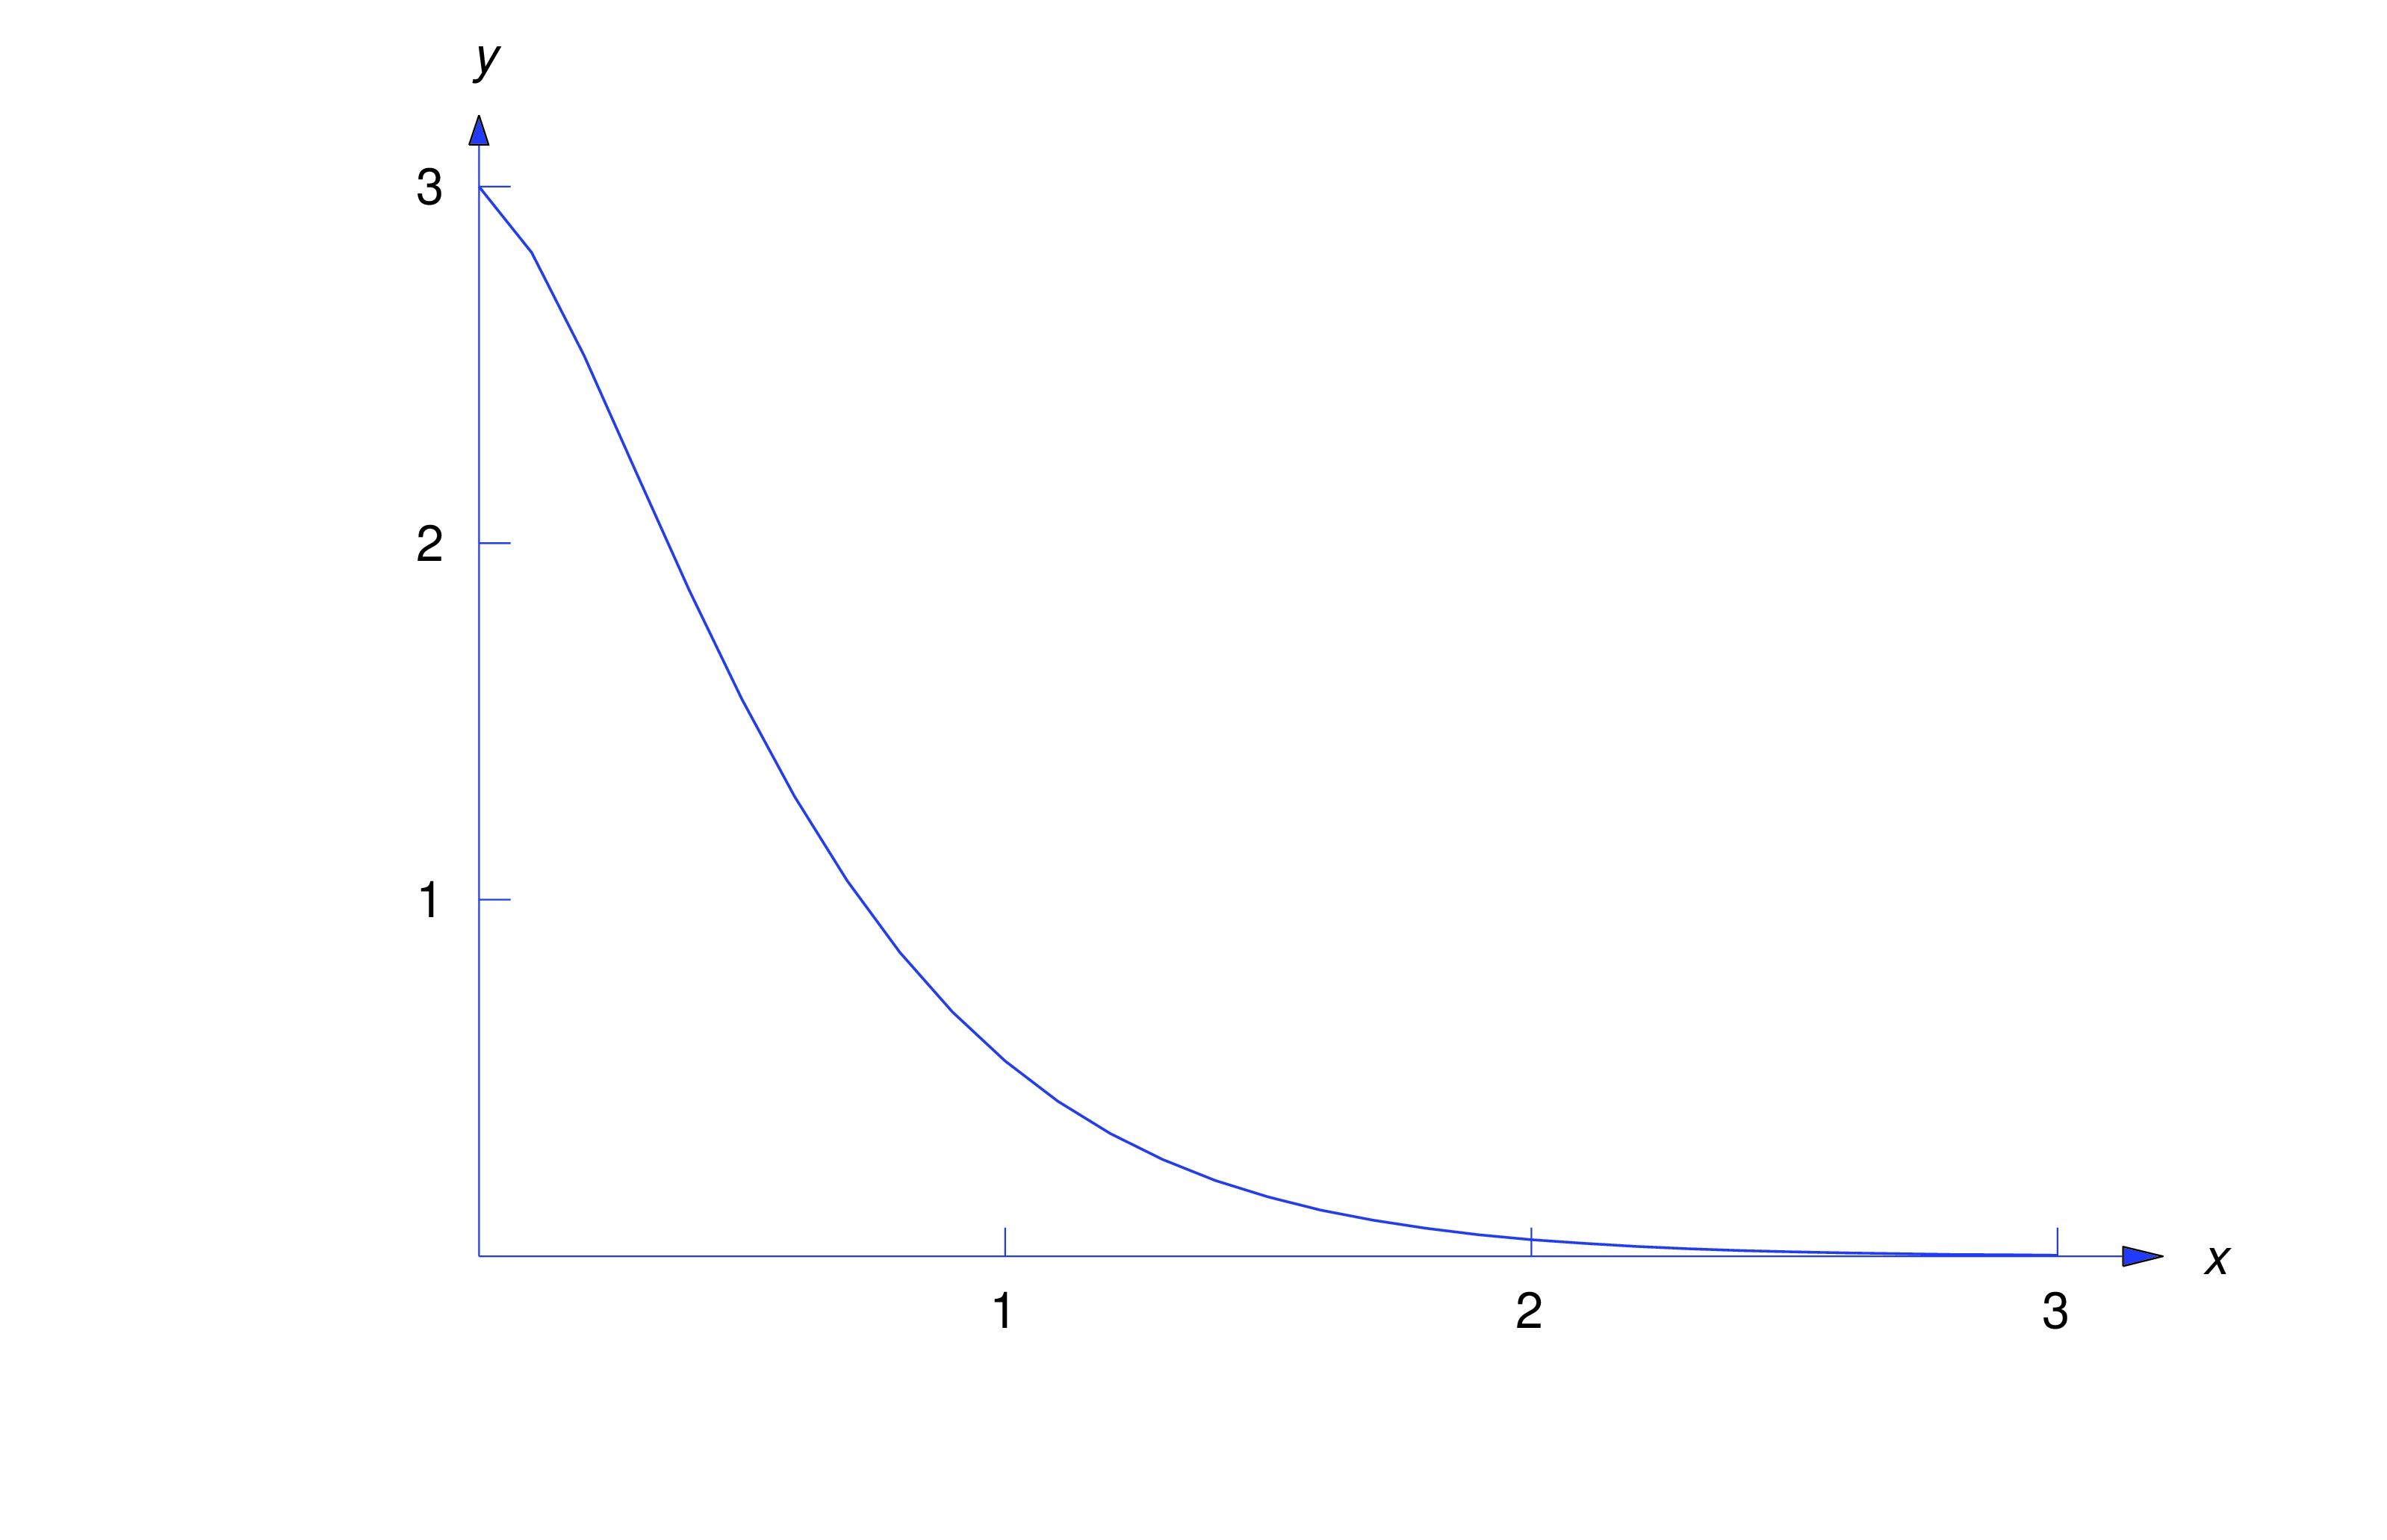
\includegraphics[height=1.5in]{fig050202.jpg}
\end{image}

\end{explanation}
\end{example}



If the characteristic equation of $ay''+by'+cy=0$
has an arbitrary repeated root $r_1$,  the
characteristic polynomial must be
$$
p(r)=a(r-r_1)^2=a(r^2-2r_1r+r_1^2).
$$
Therefore
$$
ar^2+br+c=ar^2-(2ar_1)r+ar_1^2,
$$
which implies that $b=-2ar_1$ and $c=ar_1^2$.
Therefore
 $ay''+by'+cy=0$ can be written as
$a(y''-2r_1y'+r_1^2y)=0$. Since $a\neq 0$ this equation has the same
solutions as
\begin{equation} \label{eq:5.2.12}
y''-2r_1y'+r_1^2y=0.
\end{equation}

Since $p(r_1)=0$, t $y_1=e^{r_1x}$ is a solution of
$ay''+by'+cy=0$, and therefore of \eqref{eq:5.2.12}. Proceeding as in
Example~\ref{example:5.2.2}, we look for other solutions of \eqref{eq:5.2.12}
of the form $y=ue^{r_1x}$; then
$$
y'=u'e^{r_1x}+rue^{r_1x}\quad\mbox{and}\quad
y''=u''e^{r_1x}+2r_1u'e^{r_1x}+r_1^2ue^{r_1x},
$$
so
\begin{eqnarray*}
y''-2r_1y'+r_1^2y&=&e^{rx}\left[(u''+2r_1u'+r_1^2u)-
2r_1(u'+r_1u)+r_1^2u\right]\\
&=&e^{r_1x}\left[u''+(2r_1-2r_1)u'+(r_1^2-2r_1^2+r_1^2)u\right]=u''e^{r_1x}.
\end{eqnarray*}
Therefore $y=ue^{r_1x}$ is a solution of \eqref{eq:5.2.12} if and only if
$u''=0$, which is equivalent to $u=c_1+c_2x$, where $c_1$ and $c_2$
are constants. Hence, any function of the form
\begin{equation} \label{eq:5.2.13}
y=e^{r_1x}(c_1+c_2x)
\end{equation}
is  a solution of \eqref{eq:5.2.12}.
Letting $c_1=1$ and $c_2=0$ here yields the solution
 $y_1=e^{r_1x}$ that we already knew. Letting $c_1=0$ and $c_2=1$
yields the second solution $y_2=xe^{r_1x}$. Since
$y_2/y_1=x$
is nonconstant, \ref{thmtype:5.1.6} implies that   $\{y_1,y_2\}$ is
a fundamental set of solutions of \eqref{eq:5.2.12}, and \eqref{eq:5.2.13}
is the general solution.


\subsection*{Case 3: Complex Conjugate Roots}

\begin{example}\label{example:5.2.3}
\begin{enumerate}
\item \label{item:5.2.3a}%(a)
Find the general solution of
\begin{equation} \label{eq:5.2.14}
y''+4y'+13y=0.
\end{equation}

\item \label{item:5.2.3b}%(b)
Solve the initial value problem
\begin{equation} \label{eq:5.2.15}
y''+4y'+13y=0, \quad   y(0)=2,  y'(0)=-3.
\end{equation}
\end{enumerate}

\begin{explanation}
\ref{item:5.2.3a} The characteristic
polynomial of
 \eqref{eq:5.2.14} is
$$
p(r)=r^2+4r+13=r^2+4r+4+9=(r+2)^2+9.
$$
The roots of the characteristic equation are $r_1=-2+3i$ and
$r_2=-2-3i$. By analogy with Case 1, it's reasonable to expect that
$e^{(-2+3i)x}$ and $e^{(-2-3i)x}$ are solutions of \eqref{eq:5.2.14}. This
is true %(see Exercise~\ref{exer:5.2.34});     
however, there are
difficulties here, since you are probably not familiar with
exponential functions with complex arguments, and even if you are, it's
 inconvenient to work with them, since they are complex--valued. We'll
 take a simpler approach, which we motivate as follows: the
exponential notation suggests that
$$
e^{(-2+3i)x}=e^{-2x}e^{3ix}\quad\mbox{and}\quad
e^{(-2-3i)x}=e^{-2x}e^{-3ix},
$$
so even though we haven't defined $e^{3ix}$ and $e^{-3ix}$, it's
reasonable to expect that every linear
combination of $e^{(-2+3i)x}$ and $e^{(-2-3i)x}$ can be written as
$y=ue^{-2x}$, where $u$ depends upon $x$. To determine $u$, we note
that if $y=ue^{-2x}$ then
$$
y'=u'e^{-2x}-2ue^{-2x}\mbox{\quad and \quad}
y''=u''e^{-2x}-4u'e^{-2x}+4ue^{-2x},
$$
so
\begin{eqnarray*}
y''+4y'+13y&=&e^{-2x}\left[(u''-4u'+4u)+4(u'-2u)+13u\right]\\
&=&e^{-2x}\left[u''-(4-4)u'+(4-8+13)u\right]=e^{-2x}(u''+9u).
\end{eqnarray*}
Therefore $y=ue^{-2x}$ is a solution of \eqref{eq:5.2.14} if and only if
$$
u''+9u=0.
$$
From Example~\ref{example:5.1.2}, the  general solution of this equation is
$$
u=c_1\cos 3x +c_2\sin 3x.
$$
 Therefore any function of the form
\begin{equation} \label{eq:5.2.16}
y=e^{-2x}(c_1\cos 3x+c_2\sin 3x)
\end{equation}
is  a solution of \eqref{eq:5.2.14}.
Letting $c_1=1$ and $c_2=0$  yields the solution
 $y_1=e^{-2x}\cos3x$. Letting $c_1=0$ and $c_2=1$
yields the second solution $y_2=e^{-2x}\sin3x$. Since
$y_2/y_1=\tan3x$
is nonconstant, \ref{thmtype:5.1.6} implies that   $\{y_1,y_2\}$ is
a fundamental set of solutions of \eqref{eq:5.2.14}, and \eqref{eq:5.2.16}
is the general solution.

\ref{item:5.2.3b}   Imposing the condition $y(0)=2$
in   \eqref{eq:5.2.16} shows that $c_1=2$.  Differentiating
\eqref{eq:5.2.16} yields
$$
y'=-2e^{-2x}(c_1\cos 3x+c_2\sin 3x) +3e^{-2x}(-c_1\sin 3x +c_2\cos 3x),
$$
and imposing the initial condition $y'(0)=-3$ here yields
$-3=-2c_1+3c_2=-4+3c_2$,
 so $c_2=1/3$. Therefore the solution of
\eqref{eq:5.2.15} is
$$
y=e^{-2x}(2\cos 3x+ \frac{1}{3}\sin 3x).
$$
The figure below is a graph of this function.

\begin{image}
 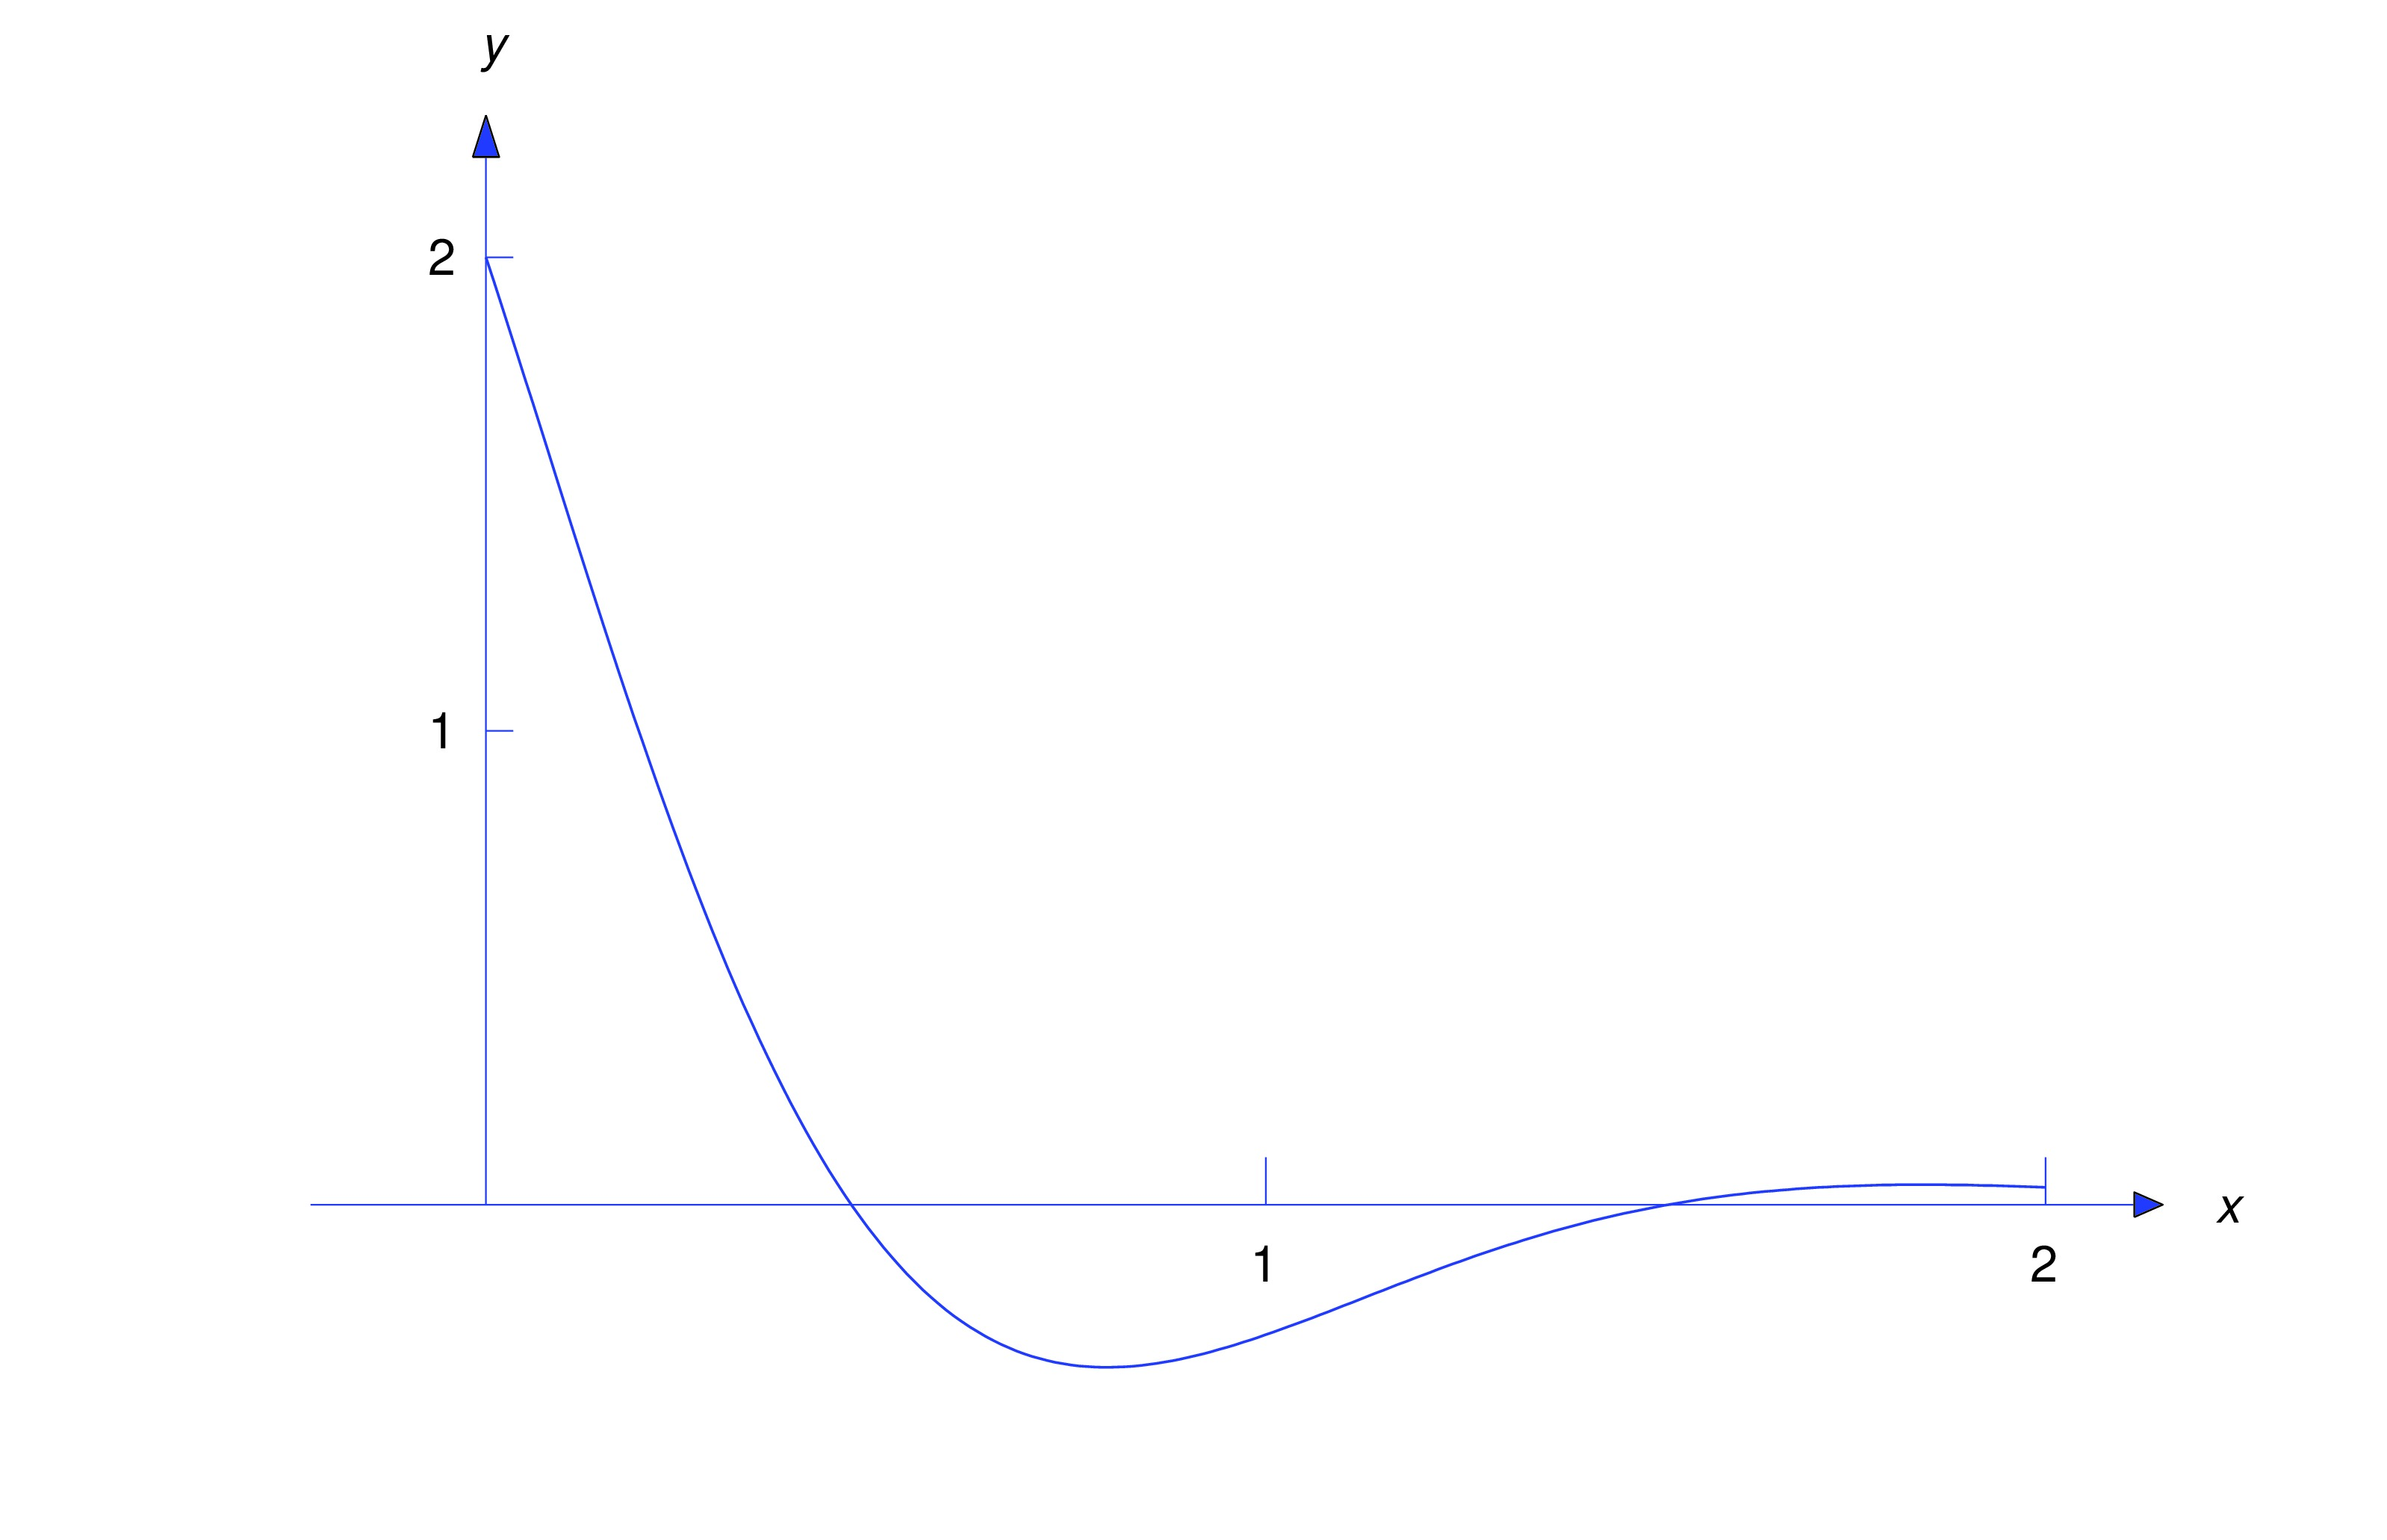
\includegraphics[height=1.5in]{fig050203.jpg}
 \end{image}
\end{explanation}
\end{example}


Now suppose   the characteristic equation of $ay''+by'+cy=0$ has
arbitrary complex roots;   thus, $b^2-4ac<0$ and, from \eqref{eq:5.2.3},
the
roots are
$$
r_1 = \frac{-b+i\sqrt{4ac-b^2}}{2a},\quad r_2 =
\frac{-b-i\sqrt{4ac-b^2}}{2a},
$$
which we rewrite as
\begin{equation} \label{eq:5.2.17}
r_1=\lambda+i \omega,\quad r_2 = \lambda - i \omega,
\end{equation}
 with
$$
\lambda = -\frac{b}{2a},\quad \omega = \frac{\sqrt{4ac-b^2}}{2a}.
$$
Don't memorize these formulas. Just remember that $r_1$
and $r_2$ are of the form \eqref{eq:5.2.17},
where  $\lambda$ is an arbitrary real number and $\omega$
is   positive;
 $\lambda$ and $\omega$ are  the \textit{real}
and \textit{imaginary parts}, respectively, of $r_1$.
Similarly, $\lambda$ and $-\omega$ are the real and imaginary parts of
$r_2$. We say that $r_1$ and $r_2$ are \textit{complex conjugates},
which means that they have the same real part and their imaginary
parts have the same absolute values, but opposite signs.

As in Example~\ref{example:5.2.3}, it's reasonable to
to expect that the solutions of $ay''+by'+cy=0$  are linear
combinations of
$e^{(\lambda+i\omega)x}$ and $e^{(\lambda-i\omega)x}$.
Again,  the exponential notation suggests that
$$
e^{(\lambda+i\omega)x}=e^{\lambda x}e^{i\omega x}\quad\mbox{and}\quad e^{(\lambda-i\omega)x}=e^{\lambda x}e^{-i\omega x}
$$
so even though we haven't defined $e^{i\omega x}$ and
$e^{-i\omega x}$, it's reasonable to expect that every linear
combination of $e^{(\lambda+i\omega)x}$ and $e^{(\lambda-i\omega)x}$
can  be written as
$y=ue^{\lambda x}$, where $u$ depends upon $x$.
To determine $u$ we first observe that since $r_1=\lambda+i\omega$
and $r_2=\lambda-i\omega$ are the roots of the characteristic
equation,  $p$ must be of  the form
$$
\begin{array}{ccl}
p(r)&=&a(r-r_1)(r-r_2)\\
&=&a(r-\lambda-i\omega)(r-\lambda+i\omega)\\
&=& a \left[(r-\lambda)^2+\omega^2\right]\\
&=&a(r^2-2\lambda r +\lambda^2+\omega^2).
\end{array}
$$
Therefore $ay''+by'+cy=0$ can be written as
$$
a\left[y''-2\lambda y'+(\lambda^2+\omega^2)y\right]=0.
$$
 Since $a\neq 0$
this equation has the same solutions as
\begin{equation} \label{eq:5.2.18}
y''-2\lambda y'+(\lambda^2+\omega^2)y=0.
\end{equation}
 To determine $u$ we note
that if $y=ue^{\lambda x}$ then
$$
y'=u'e^{\lambda x}+\lambda ue^{\lambda x}\quad\mbox{and}\quad
y''=u''e^{\lambda x}+2\lambda u'e^{\lambda x}+\lambda^2ue^{\lambda x}.
$$
Substituting these expressions  into
\eqref{eq:5.2.18} and dropping the common factor $e^{\lambda x}$ yields
$$
(u''+2\lambda u'+\lambda^2 u)-2\lambda(u'+\lambda u)
+(\lambda^2+\omega^2)u=0,
$$
which simplifies to
$$
u''+\omega^2 u=0.
$$
From Example~\ref{example:5.1.2}, the  general solution of this
equation is
$$
u=c_1\cos\omega x +c_2\sin\omega x.
$$
 Therefore any function of the form
\begin{equation} \label{eq:5.2.19}
y=e^{\lambda x}(c_1\cos\omega x+c_2\sin\omega x)
\end{equation}
is  a solution of \eqref{eq:5.2.18}.
Letting $c_1=1$ and $c_2=0$ here yields the solution
 $y_1=e^{\lambda x}\cos\omega x$. Letting $c_1=0$ and $c_2=1$
yields a second solution $y_2=e^{\lambda x}\sin\omega x$. Since
$y_2/y_1=\tan\omega x$
is nonconstant, so  Theorem~\ref{thmtype:5.1.6} implies that
$\{y_1,y_2\}$ is
a fundamental set of solutions of \eqref{eq:5.2.18}, and \eqref{eq:5.2.19}
is the general solution.

The next theorem summarizes the results of this section.

\begin{theorem}\label{thmtype:5.2.1}
Let $p(r)=ar^2+br+c$ be the characteristic polynomial of
\begin{equation} \label{eq:5.2.20}
ay''+by'+cy=0.
\end{equation}
Then:
\begin{enumerate}
\item % (a)
If $p(r)=0$  has distinct real roots $r_1$ and $r_2,$ then the general
solution of $\eqref{eq:5.2.20}$ is
$$
y=c_1e^{r_1x}+c_2e^{r_2x}.
$$
\item % (b)
If $p(r)=0$  has a repeated root  $r_1,$ then
the general solution of $\eqref{eq:5.2.20}$ is
$$
y=e^{r_1x}(c_1+c_2x).
$$
\item % (c)
If $p(r)=0$  has complex conjugate roots $r_1=\lambda+i\omega$ and
$r_2=\lambda-i\omega$ $($where $\omega>0),$ then the general solution
of $\eqref{eq:5.2.20}$ is
$$
y=e^{\lambda x}(c_1\cos\omega x+c_2\sin\omega x).
$$
\end{enumerate}
\end{theorem}

\section*{Text Source}
Trench, William F., "Elementary Differential Equations" (2013). Faculty Authored and Edited Books \& CDs. 8. (CC-BY-NC-SA)

\href{https://digitalcommons.trinity.edu/mono/8/}{https://digitalcommons.trinity.edu/mono/8/}


\end{document}